\documentclass[./\jobname.tex]{subfiles}
\begin{document}
%
\chapter{Aufgabenstellung}
%
Als Aufgabe sollen die Abweichungen der differentiellen Rückwärtskinematik von der exakten Bahn bei einer linearen Trajektorie bei drei verschiedenen Interpolationstakten \(t\_ipo = 0.1~s, \,0.01~s,\, 0.001~s\) gezeigt werden.\par
%
Folgende Schritte sollen gemacht werden:
\begin{enumerate}
\item Finden Sie eine geeignete Trajektorie, die zur Gänze im Arbeitsraum liegt und die keine Singularitäten aufweist. Es ist empfehlenswert die Trajektorie so zu wählen, dass Sie auch nicht extrem knapp an einer Singularität vorbei fährt.\par
Die Trajektorie soll mindestens 1000 mm lang sein. Vom Start zum Endpunkt sollen sich mindestens zwei Koordinaten der Position und mindestens ein Eulerwinkel ändern.\par
Verwenden Sie für \(v_{c} = 250~mm/s\) und für \(a_{max} = 250~mm/s^{2}\).\par
Vor der Ausführung der Trajektorie befindet sich der Roboter im Startpunkt in Ruhe (\(v = 0\)). Nach Ausführung der Trajektorie bleibt der Roboter im Endpunkt und verharrt in Ruhe (\(v = 0\)).\par
Halten Sie die von Ihnen verwendeten Euler-Koordinaten (\(x,y,z,\alpha,\beta,\gamma\)) des Start- und Endpunktes (in \(mm\) bzw. deg.) am Anfang Ihrer schriftlichen Ausarbeitung fest.
\item Skizzieren Sie den grundlegenden Ablauf, den Sie zur Berechnung der Ergebnisse verwendet haben (was müssen Sie wie und woraus berechnen?)
z. B. Flowchart oder Struktogramm mit den verwendeten Matlabroutinen, etc.
\item Zeichnen Sie für jeden Achswinkel ein Diagramm, in dem Sie den zeitlichen Verlauf des exakten Achswinkels (Berechnung aus der Rückwärtskinematik) mit den drei Verläufen, die Sie durch die differentielle Rückwärtskinematik ermittelt haben, gegenüber stellen (6 Diagramme mit je 4 Kurven).
\item Zeichnen Sie für die Position und Orientierung des Endeffektors (Flansch) die Diagramme, in denen Sie den zeitlichen Verlauf der x-, y- und z-Koordinate, sowie der drei Eulerwinkel der Trajektorie mit den Verläufen, die sich mit der differentiellen Rückwärtskinematik ergeben, gegenüberstellen (6 Diagramme mit je 4 Kurven).
\item Ermitteln Sie den zeitlichen Verlauf der euklidischen Distanz zwischen der exakten Position (nur \(x,y,z\)) und den Positionen, die sich durch die differentielle Rückwärtskinematik ergeben (1 Diagramm mit 3 Kurven).
\end{enumerate}
%
In der \autoref{tab: trajektorien} sind 2 Beispiele angeführt, wie Ihre Trajektorie aussehen könnte.\par
Bei Nr. 1 ändern sich alle 6 Koordinaten vom Anfangs- zum Endpunkt.
Bei Nr. 2 ändern sich nur \(x,y\) und \(z\), die Eulerwinkel bleiben konstant.
%
\begin{table}[H]
	\centering
	\noindent\adjustbox{max width=\textwidth}{%falls größer als \textwidth, wird das Bild verkleinert
	\begin{tabular}{|l|l|l|l|}
		\hline
		\rowcolor[HTML]{EFEFEF} 
		Nr. &                          & Startpunkt                  & Endpunkt                     \\ \hline
		1   & Beispieltrajektorie      & 1000, 0, 1000, 0, 95, 35    & 0, 1000, 500, -45, 175, 0    \\ \hline
		2   & Vereinfachte Trajektorie & 1000, 0, 1000, 0, 175, 0    & 0, 1000, 500, 0, 175, 0      \\ \hline
	\end{tabular}}
	\caption{Trajektorien}
	\label{tab: trajektorien}
\end{table}
%
\chapter{Ausführung}
%
\section{Trajektorienermittlung}
%
In \autoref{tab: trajektorien gefunden} ist die empirisch ermittelte Trajektorie dargestellt. Sie verläuft über einen Weg von mehr als \(1100~mm\).
%
\begin{table}[H]
	\centering
	\noindent\adjustbox{max width=\textwidth}{%falls größer als \textwidth, wird das Bild verkleinert
		\begin{tabular}{|l|l|l|l|}
			\hline
			\rowcolor[HTML]{EFEFEF} 
			Nr. &                          & Startpunkt                  & \\ \hline
			1   & Eigene Trajektorie       & 700, -750, 500, 0, 160, -85 & 1000, 250, 1000, 0, 100, -25 \\ \hline
	\end{tabular}}
	\unterschrift{Trajektorie ermittelt}{eigene Ausarbeitung}{}
	\label{tab: trajektorien gefunden}
\end{table}
%
In \autoref{fig: robot-irb4600-path2.eps} ist der gefahrene Roboterpfad dargestellt.
%
\begin{figure}[H]
	\centering
	\noindent\adjustbox{max width=\textwidth}{%falls größer als \textwidth, wird das Bild verkleinert
		%trim option's parameter order: left bottom right top
		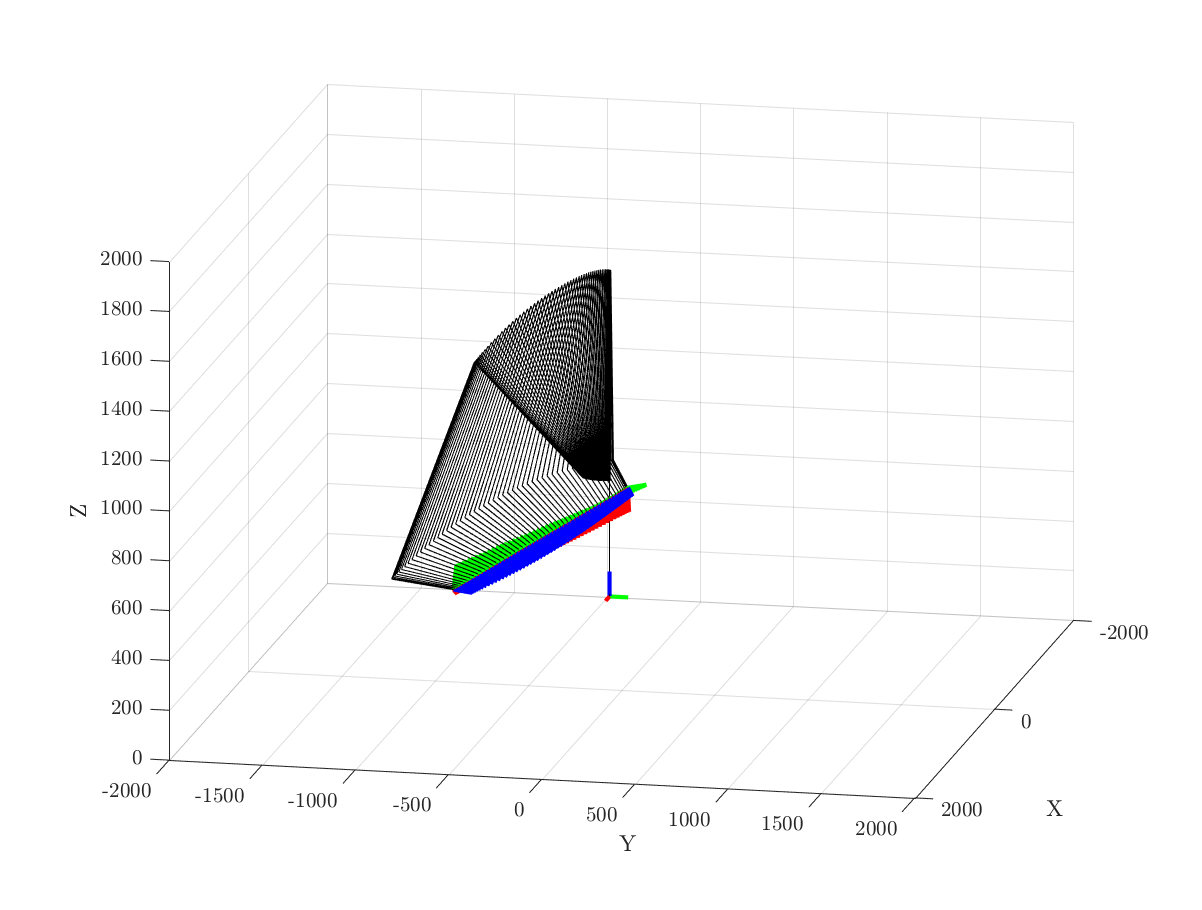
\includegraphics[width=1\textwidth]{./img/robot-irb4600-path2.eps}
	}
	\unterschrift{Roboter Pfad}{eigene Ausarbeitung}{}
	\label{fig: robot-irb4600-path2.eps}
\end{figure}
%
\section{Grundlegender Ablauf des Matlab Scripts}
%
In \autoref{fig: verwendete Variablen} sind die verwendeten Variablen und ihre Beschreibung dargestellt.
%
\def\ctrTipo{\textcolor{red}{\pVar{ctrTipo}}}
\def\kVar{\textcolor{red}{\pVar{k}}}
\def\tIpo{\textcolor{red}{\pVar{t\_ipo}}}
\def\diffQ{\textcolor{red}{\pVar{diffQ}}}
\def\ecDiff{\textcolor{red}{\pVar{ec_diff}}}
\def\vZero{\textcolor{red}{\pVar{v0}}}
\def\analyticalQ{\textcolor{red}{\pVar{analyticalQ}}}
\def\qDot{\textcolor{red}{\pVar{qDot}}}
\def\ec{\textcolor{red}{\pVar{ec}}}
\def\ecDiffRe{\textcolor{red}{\pVar{ec_diffRe}}}
\def\vNext{\textcolor{red}{\pVar{vNext}}}

\def\vonK{\(_{k}\)\xspace}
\def\vonKP{\(_{k+1}\)\xspace}
\def\vonKM{\(_{k+1}\)\xspace}
%
\begin{figure}[H] 
	\centering 
	\noindent\adjustbox{max width=\textwidth}{%falls größer als \textwidth, wird das Bild verkleinert
	\begin{struktogramm}(150,80)
		\assign{%
			\descriptionindent = .5em
			\descriptionwidth = 60pt
			\descriptionsep=0pt
			\begin{declaration}[Variablen]
				\description{\ctrTipo}{Zähler für Taktzeit.}
				\description{\kVar}{Iterationsvariable für jeden Trajektiorienschritt.}
				\description{\tIpo}{Hällt im Arrayverbund die Taktzeiten von \(0.1~s,\,0.01~s,\,0.001~s \).}
				\description{\diffQ}{Differentielle Achswinkel der sechs Achsen für die gesamte Trajektorie.}
				\description{\ecDiff}{Differentielle Trajektorie des Zielframes.}
				\description{\ecDiffRe}{Vom\analyticalQ zurück gerechnete Trajektorie des Zielframes.}
				\description{\vZero}{Enthällt die Geschwindigkeiten des Zielframes für die gesamte Trajketorie.}
				\description{\analyticalQ}{Mit der analytisch ermittelten Rückwärtskinematik gerechneten Achswinkel.}
				\description{\qDot}{Ableitungen der differentiellen Achswinkel für die gesamte Trajektorie.}
				\description{\ec}{Solltrajektorie.}
			\end{declaration}
		}
	\end{struktogramm}}
	\unterschrift{Matlab Script: verwendete Variablen}{eigene Ausarbeitung}{}
	\label{fig: verwendete Variablen}
\end{figure}
%
In \autoref{fig: programm logik} ist die Programmlogik dargestellt und beschrieben. Der Matlab Code für die Berechnung ist in \autoref{chap: matlab code} zu finden.
%
\begin{figure}[H] 
	\centering 
	\noindent\adjustbox{max width=\textwidth}{%falls größer als \textwidth, wird das Bild verkleinert
	\begin{struktogramm}(160,245)
		\assign{\ctrTipo \(\gets 1\)}
		\while[1]{\ctrTipo <= length(\tIpo)}
		%\assign[\abstand]{create\_lin\_seg\_list()}
		%\assign[\abstand]{create\_lin\_intvec()}
		\assign[\abstand]{create\_lin\_seg\_list() 
		\\ \pComment{Beschleunigungszeiten und Beschleunigung berechnen.}\\
		create\_lin\_intvec()
		\\ \pComment{für jeden Zeitschritt \(t\) \(s,x,a\) berechnen.}\\
			\ec = create\_lin\_path()
			\\ \pComment{die Solltrajektorie berechnen.}
		}
		\assign[\abstand]{Variablen Speicher allozieren \pfeil ist schneller!}
		\assign{\kVar \(\gets 1\)}
		\while[1]{\kVar \(\leq\) length(\ec)}
		\assign[\abstand]{tg = xyzabc\_2\_t(\ec\vonK) 
		\\\pComment{Zielframe berechnen von der Trajektorie.}}
		\assign[\abstand]{\analyticalQ\vonK = irb4600\_rk(tg, robot) \\\pComment{Analytische Rückwärtskinematik zum Vergleich berechnen.}}
		\assign[\abstand]{coor\_wRe = fk\_craig(\analyticalQ\vonK, robot) \\ \\\pComment{Zurückrechnen auf den Zielframe}}
		\assign[\abstand]{\ecDiffRe\vonK = t\_2\_xyzabc(coor\_wRe, 1) \\\pComment{Zurückrechnen vom Zielframe auf die Trajektorie.}}
		\ifthenelse[10]{2}{4}
		{\kVar == 1}{\sFalse}{\sTrue}%
		
		%\sub{\(\color{orange}m \gets 0\)}
		%\assign[\abstand]{Zeile inkrementieren}
		%\sub{\(\color{green}n \gets n + 1\)}
		\change
		\assign[\abstand]{\vZero\vonK = 0}
		\assign[\abstand]{\vNext\vonK = 0}
		\assign[\abstand]{\diffQ\vonK = \analyticalQ\vonK \\ \pComment{Erste Achswinkel von der Rückwärtskinematik nehmen, da keine Wegmessung in der Simulation integriert ist.}}
		%\assign[\abstand]{coor\_w=fk\_craig(\diffQ\vonK,robot) \\\pComment{Zielframe von den differentiellen Achswinkeln berechnen.}}
		%\assign[\abstand]{\(actualEC_{k} = ec_{k}\) \pComment{Solltrajektorie vorbereiten zur Übergabe.}}
		%\assign{\( n \gets 1\)}
		%		\while[1]{\(\color{red}n <= length(trajektNext)\)}
%		\assign[\abstand]{
%			\vNext\vonK= \ec\vonK \(-\) \ec\vonKM \tIpo(\ctrTipo)
%			\\\pComment{
%				Differentiell die Geschwindigkeiten ausrechnen für \(v_{x},v_{y},v_{z},\dot{\alpha},\dot{\beta},\dot{\gamma}\) mittels der Solltrajektorie.}
%		}
		%\whileend
		\ifend
		\assign[\abstand]{coor\_w=fk\_craig(\diffQ\vonK,robot) \\\pComment{Zielframe von den differentiellen Achswinkeln berechnen.}}
		\assign[\abstand]{\ecDiff\vonK=t\_2\_xyzabc(coor\_w, 1) \\\pComment{mithilfe des Zielframes der Differentiellen Rückwärtskinematik, die differentielle Trajektorie bestimmen.}}
		
		\ifthenelse[10]{2}{4}
		{\kVar > 1}{\sFalse}{\sTrue}%
%		\assign[\abstand]{\pComment{Anfangswerte Initialisieren}}
		%\sub{\(\color{orange}m \gets 0\)}
		%\assign[\abstand]{Zeile inkrementieren}
		%\sub{\(\color{green}n \gets n + 1\)}
		\change
		%\assign[\abstand]{\(actualEC_{k} = ec_{k}\) \pComment{Solltrajektorie vorbereiten zur Übergabe.}}
		%\assign{\( n \gets 1\)}
		%		\while[1]{\(\color{red}n <= length(trajektNext)\)}
		\assign[\abstand]{
			\vNext\vonK= \ec\vonK \(-\) \ec\vonKM \tIpo(\ctrTipo)
			\\\pComment{
				Differentiell die Geschwindigkeiten ausrechnen für \(v_{x},v_{y},v_{z},\dot{\alpha},\dot{\beta},\dot{\gamma}\) mittels der Solltrajektorie.}
		}
		%\whileend
		\ifend
		
		\assign[\abstand]{omega = deg2rad(abc\_t\_w(\ec\vonK, \vNext\vonK(\(\dot{\alpha},\dot{\beta},\dot{\gamma}\)))) \\\pComment{Mithilfe der aktuellen Position in \(x,y,z\) und \(\dot{\alpha},\dot{\beta},\dot{\gamma}\) berechnet sich omega in Radiant.}}
		\assign[\abstand]{\vZero\vonK = \vNext\vonKP \& omega
		\\ \pComment{v0 richtig zusammenstellen aus \(x,y,z\) und omega.}}
		\assign[\abstand]{\qDot\(_{k}\) = rad2deg(irb4600\_jakobi(\diffQ\vonK)\(^{-1} \cdot\) \vZero\vonK)
		\\ \pComment{mithilfe der IRB4600 Jakobi und v0 die Ableitungen der Achswinkel berechnen.}}
		\assign[\abstand]{\diffQ\vonKP = \diffQ\vonK + \qDot\vonK \(\cdot\) \tIpo(\ctrTipo)
		\\ \pComment{differentielle Achswinkel für nächsten Zyklus berechnen.}}
		\assign[\abstand]{\(x_{dif} = \left(\text{\ecDiff}(x_{k})-\text{\ec}(x_{k-1})\right)\)\\
			\(y_{dif}=\left(\text{\ecDiff}(y_{k})-\text{\ec}(y_{k-1})\right)\)\\
			\(z_{dif}= \left(\text{\ecDiff}(z_{k})-\text{\ec}(z_{k-1})\right)\)\\
			euklAbstand=\(\sqrt{
				x_{dif}^{2}+ 
				y_{dif}^{2} + z_{dif}^{2}
			}  \)
		\\\pComment{euklidischer Abstand berechnen.}}
		\assign[\abstand]{\kVar++}
		\whileend
		\assign[\abstand]{\ctrTipo++}
		\whileend
	\end{struktogramm}}
	\unterschrift{Matlab Script Logik}{eigene Ausarbeitung}{}
	\label{fig: programm logik}
\end{figure}
%
\section{Verlauf der Achswinkel}
%
\begin{figure}[H]
	\centering
	\noindent\adjustbox{max width=\textwidth}{%falls größer als \textwidth, wird das Bild verkleinert
		%trim option's parameter order: left bottom right top
		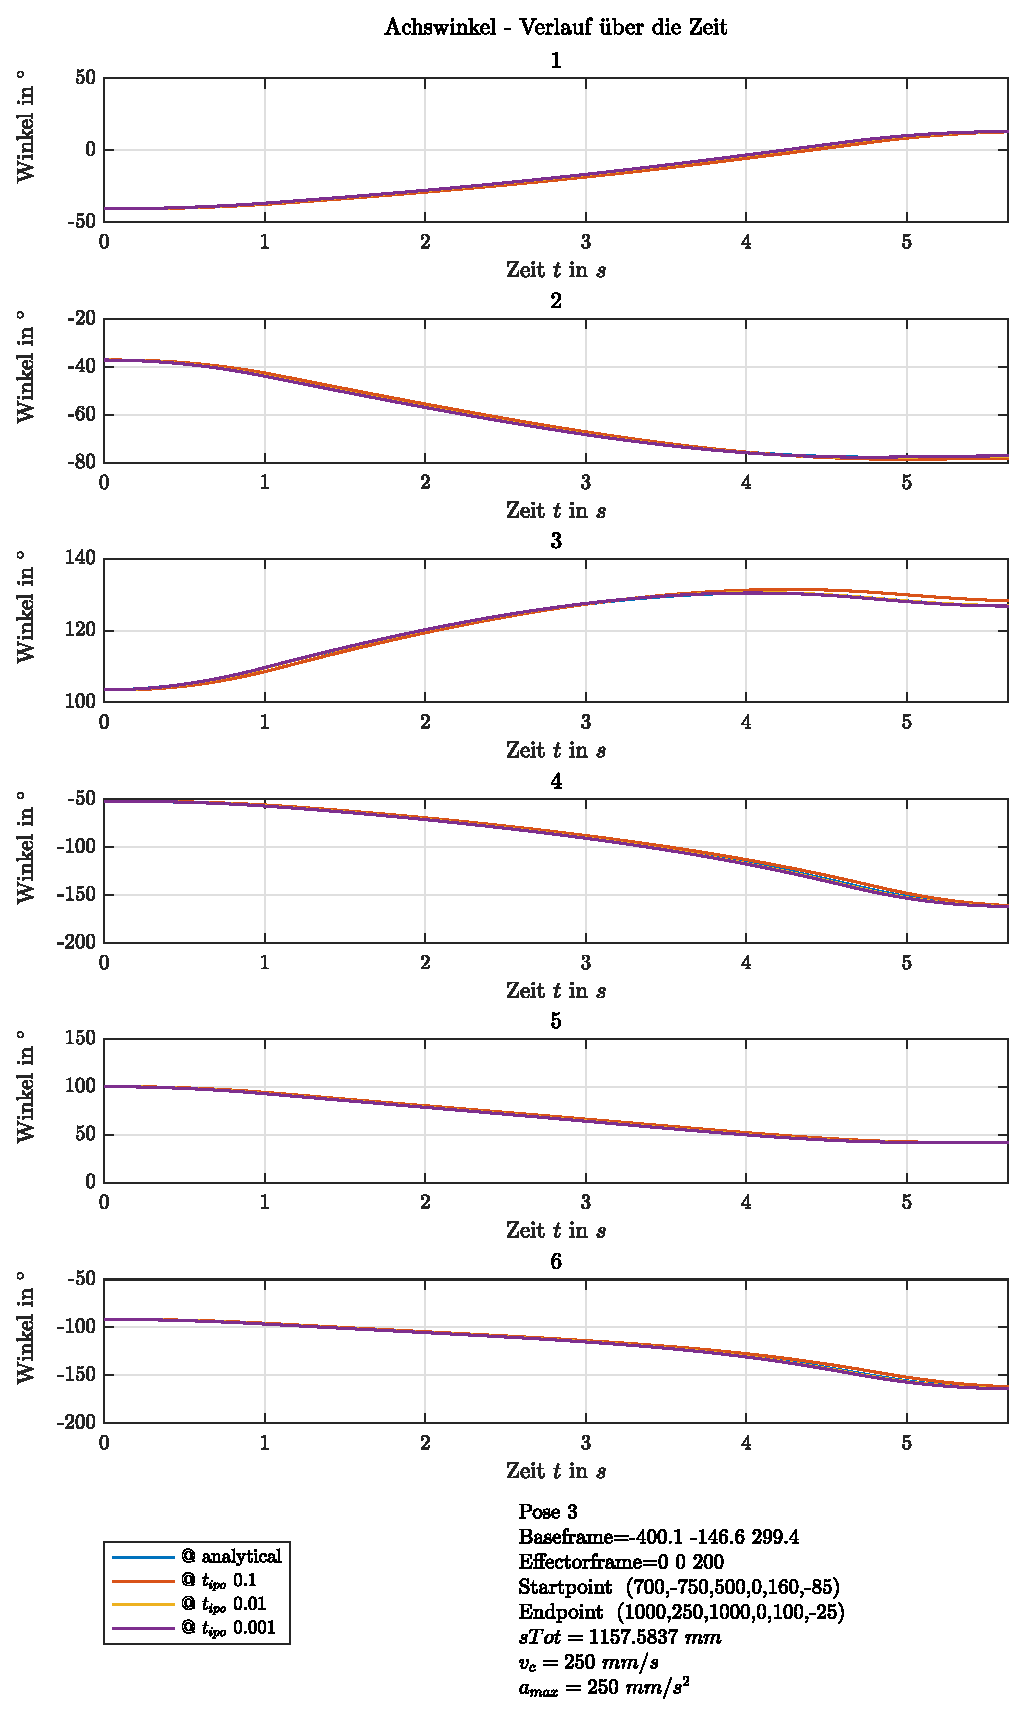
\includegraphics[width=0.85\textwidth]{./img/achswinkel2.eps}
	}
	\unterschrift{Achswinkel - Verlauf über die Zeit}{eigene Ausarbeitung}{}
	\label{fig: achswinkel1.eps}
\end{figure}
%
\section{Verlauf der Eulerkoordinaten}
%
\begin{figure}[H]
	\centering
	\noindent\adjustbox{max width=\textwidth}{%falls größer als \textwidth, wird das Bild verkleinert
		%trim option's parameter order: left bottom right top
		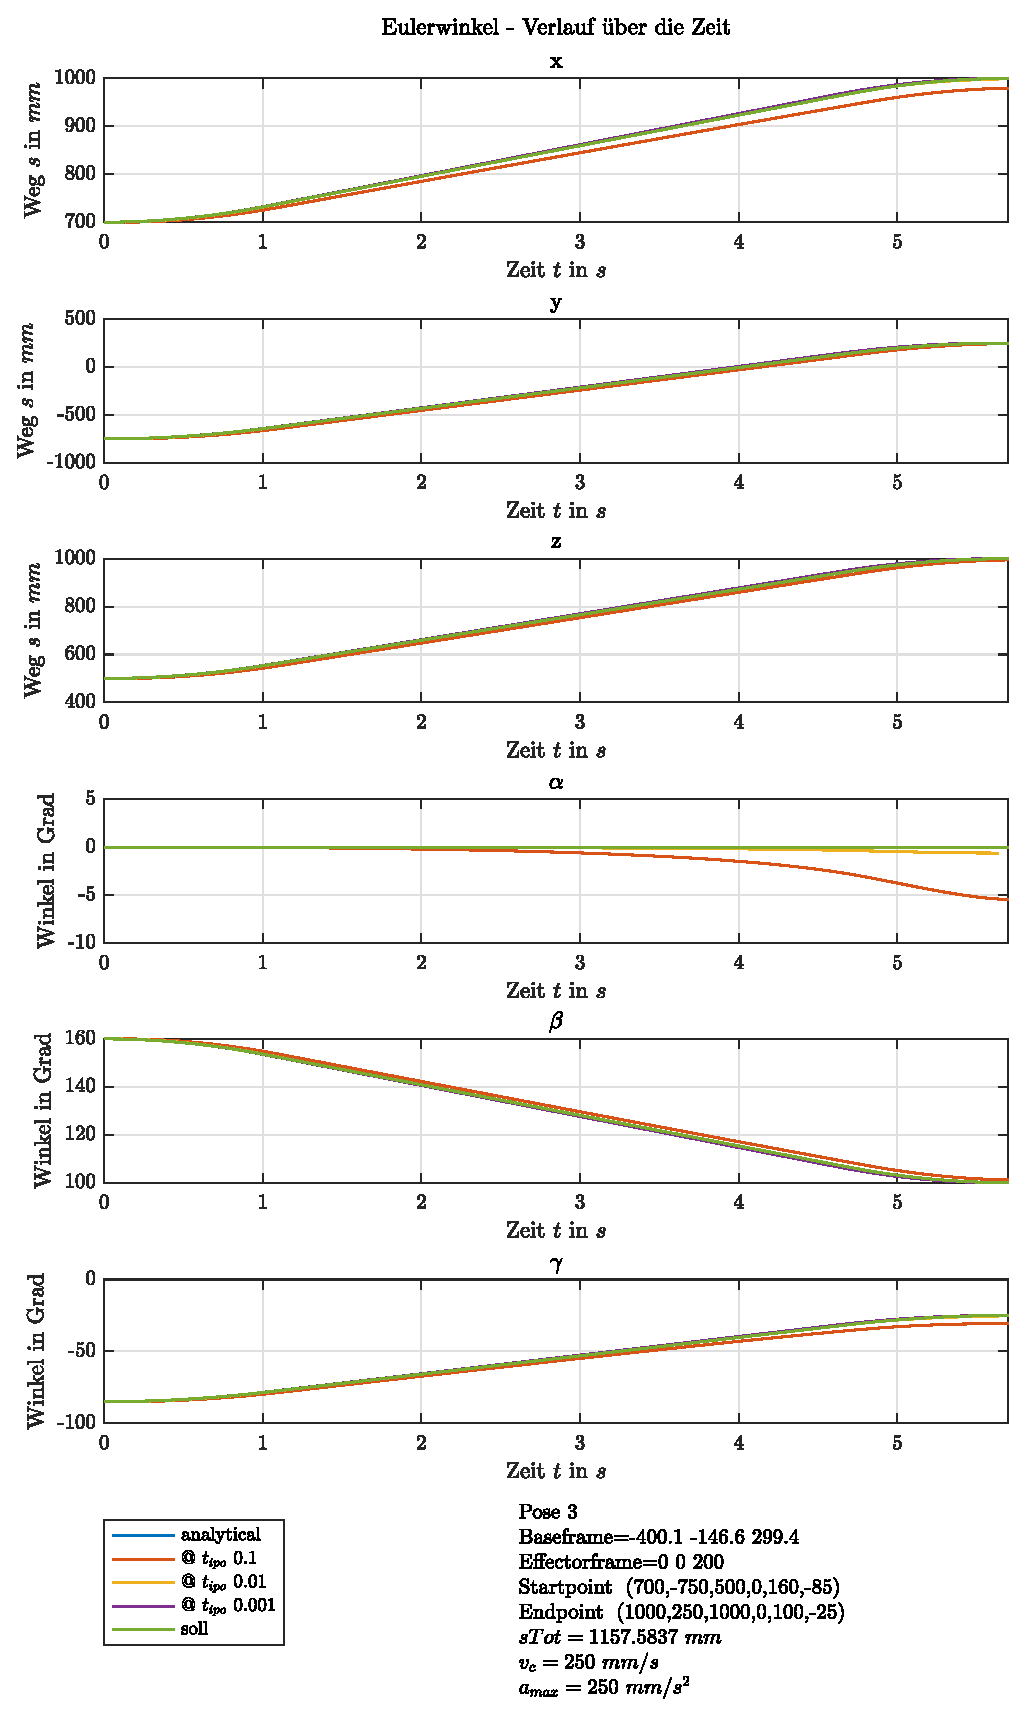
\includegraphics[width=0.85\textwidth]{./img/eulerwinkel2.eps}
	}
	\unterschrift{Eulerkoordinaten - Verlauf über die Zeit}{eigene Ausarbeitung}{}
	\label{fig: eulerwinkel1.eps}
\end{figure}
%
\section{Euklidischer Abstand}
%
\begin{figure}[H]
	\centering
	\noindent\adjustbox{max width=\textwidth}{%falls größer als \textwidth, wird das Bild verkleinert
		%trim option's parameter order: left bottom right top
		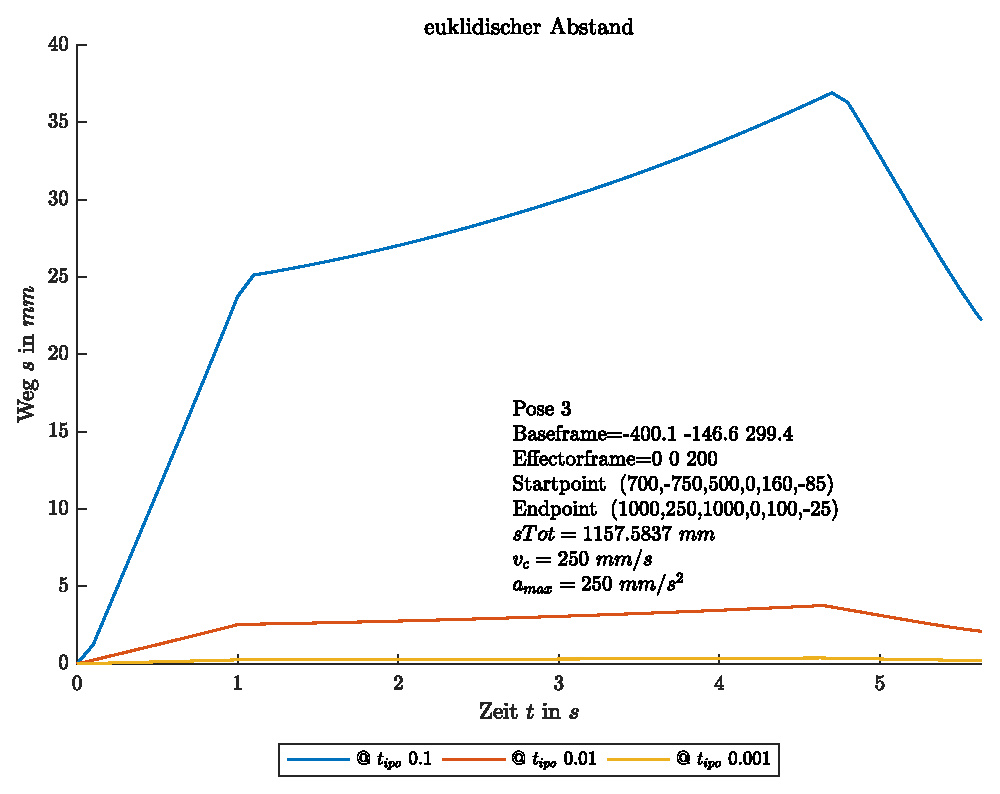
\includegraphics[width=1\textwidth]{./img/euklAbstand2.eps}
	}
	\unterschrift{euklidischer Abstand}{eigene Ausarbeitung}{}
	\label{fig: euklAbstand1.eps}
\end{figure}
%
\end{document}
